\section{Site cost estimation}

In order to be able to estimate the feasibilty of possible computing models in the future of LHC, some understanding
of computing resources costs is necessary, at a global scale.
This requires an analysis of what computing expenses are now and what they are likely to be in the coming years, based on
what we have been observing over the last years.
The main difficulty lies in the fact that various academic data centers (``sites'') contribute to WLCG, they belong
to different nations with different resource types and costs, different service levels, funding models,
strategies, energy providers and so on. This study aims to understand these differences and provide a set of indicators
that make sense for all sites.


\subsection{\label{sec:sitecost:computing}Computing resource costs}

The first major step of this approach consisted in gathering relevant indicators related to computing resource costs
from the biggest data centers partcipating in WLCG.

We first focus on the distributions of CPU, disk and tape cartridge costs for hardwares procured in 2018.
Figure~\ref{fig:sitecost} represents the obtained results and Table~\ref{tab:sitecosts} summarizes the average values
and deviation across sites. If CPU price is rather homogeneous across sites, the variance
in storage costs is quite important. This effect is due to a larger diversity of the storage technologies local market,
and unlike CPU, the performance is not benchmarked and remains harder to compare across sites.

In addition to the 2018 purchase costs, we established the evolution of the purchase cost over the years, per site,
although not all sites could provide relevant data. It is clear that CPU price evolution is not as fast as expected: all
sites oberve a slow down in CPU price evolution trend, which remains far below $-20 \%$ per year.
For disk storage, the picture is rather coherent and many sites
observed an price evolution of about $-15 \%$ per year.
Draw any conclusion from tape storage cost trend is quite difficult:
an important change in the tape and libraries market has been taking place recently, and every site is in a different
situation: we will probably stay on average below the $-20 \%$ per year for some time.


\begin{table}[h]
    \centering
    \caption{Site costs summary (as of 2018) and evolution over the previous years.}
    \label{tab:sitecosts}
    \begin{tabular}{l|rrr}
        \hline
        resource & CPU & disk & cartridge \\\hline
        average purchase cost & 10.3 \euro/HS06 & 126.5 \euro/TB & 12.8 \euro/TB \\\hline
        deviation & 26 \% & 51 \% & 57 \% \\\hline
        average trend & -12 \%/y & -15 \%/y & -14 \%/y \\\hline
        deviation & 37 \% & 20 \% & 43 \%\\\hline
    \end{tabular}
\end{table}

\begin{figure}
    \subfloat[CPU]{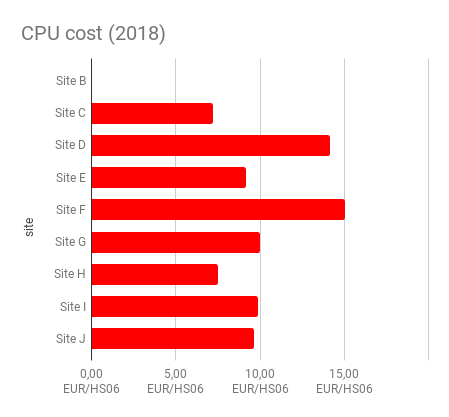
\includegraphics[width = 0.33\textwidth]{CPU_cost.png}}
    \subfloat[Disk]{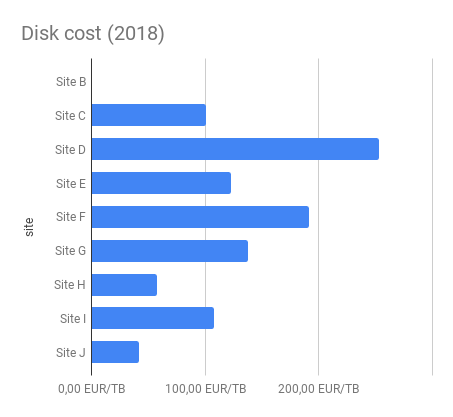
\includegraphics[width = 0.33\textwidth]{Disk_cost.png}}
    \subfloat[Tape cartridges]{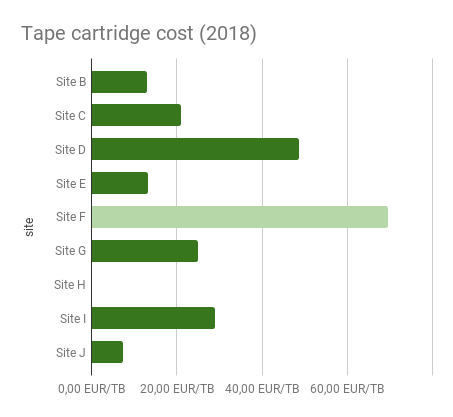
\includegraphics[width =0.33\textwidth]{Tape_cost.png}}
    \caption{Add your own figures before compiling}
    \label{fig:sitecost}
\end{figure}



\subsection{\label{sec:sitecost:energy}Energy}


\subsection{\label{sec:sitecost:tco}TCO}As a second step, we tried to estimate the total cost of ownership (TCO) of two typical data centers and classify the relative
weight of the various contributions to it

